\documentclass[a4paper, 11pt, final, garamond]{book}
\usepackage{cours-preambule}
\usepackage[french]{babel}

\raggedbottom

\makeatletter
\renewcommand{\@chapapp}{Programme de kh\^olle -- semaine}
\makeatother

\begin{document}
\setcounter{chapter}{28}

\chapter{Du 05 au 09 juin}

\section{Cours et exercices}

\section*{Thermo. chapitre 3 -- Second principe, machines thermiques}
\begin{enumerate}[label=\Roman*]
  \litem{L'entropie}
  \litem{Machines thermiques}
  \litem{Notations infinitésimales et interprétation microscopique}
\end{enumerate}

\section*{Thermodynamique chapitre 4 -- Changements d'états}
\begin{enumerate}[label=\Roman*]
  \litem{Introduction}~: vocabulaire, observation changement température fixée
    pour pression fixée, hypothèses de travail.
  \litem{Diagramme $(P,T)$}~: cas fréquent, cas rare, vocabulaire courbes
    d'équilibre diphasé, point triple, point critique, pression de vapeur
    saturante.
  \litem{Diagramme de \textsc{Clapeyron}}~: expérience compression d'un gaz et
    changement d'état liquide, forme d'une courbe en $(P,V)$, et bilan
    isothermes d'\textsc{Andrews}~: courbes de rosée et d'ébullition~; titres
    massiques et théorème des moments. Application stockage de l'eau.
  \litem{Enthalpie diphasée et de transition}~: définitions, exemple
    calorimétrie.
  \litem{Entropie diphasée et de transition}~: définitions, réversibilité,
    exemple calorimétrie.
  \litem{Machine avec transition liquide/vapeur}~: présentation machine avec
    écoulement, premier principe industriel et cas particuliers, diagramme
    $(p,h)$~: vocabulaire et cas particuliers~; modélisation d'une machine
    frigorifique, étude en diagramme $(p,h)$.
\end{enumerate}

\section{Cours uniquement}

\section*{Architecture de la matière ch.3 -- Solides cristallins}
\begin{enumerate}[label=\Roman*]
  \litem{Différents types de solides}~: solides cristallins, amorphes,
    semi-cristallins~; allotropie.
  \litem{Modèle du cristal parfait}~: description (réseau, motif, maille),
    mailles cubiques (CS, CC, CFC), dénombrement (population, coordinence),
    occupation du volume (compacité, masse volumique), limite du modèle.
  \litem{Cristal parfait de sphères dures}~: modèle, empilements compacts (ABA,
    ABC), condition de contact et application calculs de compacité (CS, CC,
    CFC), sites interstitiels (définition, habitabilité, sites O et T)~: nombre
    de sites O par maille et habitabilité. \textbf{Sites T non traités pour le
    moment}.
\end{enumerate}

\section{Questions de cours possibles}

\begin{enumerate}[label=\sqenumi]
    \item[] \textbf{Thermo. chapitre 3}

    \item Énoncer les 3 lois de \textsc{Laplace} en précisant leurs conditions
      d'application. Comment qualifier ces transformations en terme d'entropie~?
      À partir d'une expression de l'entropie pour un GP (rappelée par
      l'interrogataire), démontrer l'une d'entre elle. Retrouver les deux autres
      à partir de celle-ci. Application~: on prend \SI{20}{L} de gaz à $T =
      \SI{293}{K}$ et à \SI{1}{bar}. Sous les conditions d'application
      précédentes, on le comprime jusqu'à un volume de \SI{10}{L}. Calculer la
      pression et la température, connaissant $\gamma = \num{1.4}$.

    \item Présenter le principe général d'une machine \textbf{ditherme}.
      Démontrer les deux relations utiles pour les machines à partir du premier
      et du second principe (inégalité de \textsc{Clausius}). Pourquoi ne
      peut-on pas réaliser de moteur monotherme~? Construire le diagramme de
      \textsc{Raveau} pour les machines dithermes, en précisant les domaines des
      moteurs et des réfrigérateurs.

    \item Présenter le moteur ditherme, le réfrigérateur \textbf{ET} la pompe à
      chaleur, en différenciant les sens conventionnel et réel des échanges.
      Définir leurs efficacités thermodynamiques, donner leurs efficacités de
      \textsc{Carnot}, et établir l'efficacité de \textsc{Carnot} d'\textbf{une}
      des machines.

    \item Cycle de \textsc{Carnot}~: définir les transformations, traduire le
      vocabulaire associé, le dessiner dans un diagramme $(P,V)$, trouver le
      travail total (on admet l'expression du travail pour une isotherme
      quasi-statique~: $W_{\rm isoT} = nRT_{\rm iso} \ln \left(
      V_{i}/V_{f} \right)$), la chaleur échangée et l'expression finale
      du rendement.

    \item[] \textbf{Thermo. chapitre 4}
    \item Présenter le diagramme $(P,T)$ des transitions de phase. Présenter
      l'expérience du cours permettant de tracer une transition gaz/liquide dans
      un diagramme $(P,V)$, et la tracer dans ce diagramme en faisant
      correspondre les différentes étapes sur la courbe. Présenter alors les
      isothermes d'\textsc{Andrews}.

    \item Énoncer et démontrer le théorème des moments. Refaire l'exercice
      suivant~:
\end{enumerate}
\begin{NCexem}{Isothermes d'\textsc{Andrews}}
  \begin{minipage}[t]{.60\linewidth}
    La figure ci-contre représente un ensemble de courbes expérimentales
    appelées isothermes d'\textsc{Andrews}, représentant la pression $P$ d'une
    mole de fluide en fonction du volume \textbf{molaire}, pour différentes
    températures. \smallbreak
    \begin{enumerate}
      \item Déterminer les coordonnées $(P_C,V_C)$ du point critique.
      \item Indiquer la courbe de rosée et la courbe d'ébullition.
      \item Préciser l'état physique et calculer, s'ils sont définis, les titres
        massiques $x_V$ et $x_L$ de la vapeur et du liquide pour~:
        \begin{enumerate}
          \item $V_m = \SI{0.6}{L.mol^{-1}}$ et $T = \SI{110}{\degreeCelsius}$~;
          \item $P = \SI{110}{bars}$ et $T = \SI{200}{\degreeCelsius}$~;
          \item $V_m = \SI{0.2}{L.mol^{-1}}$ et $T = \SI{125}{\degreeCelsius}$.
        \end{enumerate}
      \item Que vaut le volume molaire de la vapeur saturante à la
        pression de \SI{40}{bars}~?
    \end{enumerate}
  \end{minipage}
  \begin{minipage}[t]{.40\linewidth}
    ~
    \vspace*{-10pt}
    \begin{center}
      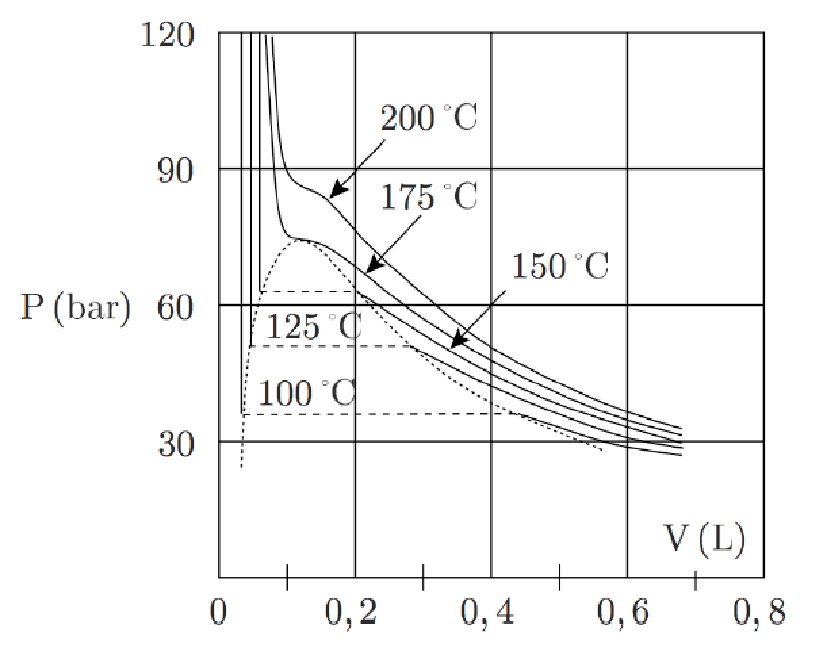
\includegraphics[scale=1]{../figures/ch29/iso_and}
      \label{fig:isoand}
    \end{center}
  \end{minipage}
\end{NCexem}
\begin{enumerate}[label=\sqenumi, resume]
  \item Exprimer une variation d'enthalpie et d'entropie pour une transition
    de phase. \textbf{Application}~: Dans un calorimètre parfaitement isolé de
    capacité thermique $C = \SI{150}{J.K^{-1}}$, on place $m = \SI{300}{g}$
    d'eau à la température $\theta = \SI{20}{\degreeCelsius}$ en équilibre
    thermique avec le vase intérieur et une masse $m_g = \SI{40}{g}$ de glace
    sèche à \SI{0}{\degreeCelsius}. Déterminer la température d'équilibre,
    sachant $c_{\rm eau} = \SI{4.185e3}{J.K^{-1}.kg^{-1}}$ et $\Delta{h_{\rm
    fus}} = \SI{330}{kJ.kg^{-1}}$. Déterminer la variation d'entropie. On
    donne que pour une phase condensée, $\Delta{S} = C \ln \left(
    \frac{T_f}{T_i} \right)$.

  \item[] \textbf{AM. chapitre 3}

  \item Présenter le modèle du cristal parfait. Présenter les mailles cubiques
    classiques. Rappeler (et démontrer) les fondamentaux de géométrie d'un cube.
    Définir la population, la coordinence, la compacité et la masse volumique.
    Présenter le modèle des sphères dures, la condition de tangence et indiquer
    l'endroit de tangence pour les 3 mailles cubiques.

  \item Décrire la maille cubique faces centrées. Déterminer sa population, sa
    coordinence, sa compacité. \textbf{Application}~: le fer $\gamma$ est une
    variété allotropique du fer, cristallisant dans une structure CFC. Sa masse
    volumique vaut $\rho = \SI{8.21e3}{kg.m^{-3}}$. Déterminer le paramètre de
    la maille $a$ et de rayon $r$ des atomes de fer dans la structure. On donne
    $M_{\ce{Fe}} = \SI{56}{g.mol^{-1}}$ et $\mathcal{N}_A =
    \SI{6.02e23}{mol^{-1}}$.

  \item Présenter et justifier l'existence des sites interstitiels. Donner les
    positions et la population des sites O de la structure CFC, et déterminer
    leur habitabilité.
\end{enumerate}

\begin{center}
  \begin{framed}
    \Huge Au moins deux questions de cristallographie pour un groupe de trois.
  \end{framed}
\end{center}

\end{document}
